%%%%%%%%%%%%%%%%%%%%%%%%%%%%%%%%%%%%%%%%%
% Journal Article
% LaTeX Template
% Version 1.4 (15/5/16)
%
% This template has been downloaded from:
% http://www.LaTeXTemplates.com
%
% Original author:
% Frits Wenneker (http://www.howtotex.com) with extensive modifications by
% Vel (vel@LaTeXTemplates.com)
%
% License:
% CC BY-NC-SA 3.0 (http://creativecommons.org/licenses/by-nc-sa/3.0/)
%
%%%%%%%%%%%%%%%%%%%%%%%%%%%%%%%%%%%%%%%%%

%----------------------------------------------------------------------------------------
%	PACKAGES AND OTHER DOCUMENT CONFIGURATIONS
%----------------------------------------------------------------------------------------

 \documentclass[twoside,twocolumn]{article}

\usepackage{blindtext} % Package to generate dummy text throughout this template 

\usepackage[sc]{mathpazo} % Use the Palatino font
\usepackage[T1]{fontenc} % Use 8-bit encoding that has 256 glyphs
\linespread{1.05} % Line spacing - Palatino needs more space between lines
\usepackage{microtype} % Slightly tweak font spacing for aesthetics

\usepackage[english]{babel} % Language hyphenation and typographical rules

\usepackage[hmarginratio=1:1,top=32mm,columnsep=20pt]{geometry} % Document margins
\usepackage[hang, small,labelfont=bf,up,textfont=it,up]{caption} % Custom captions under/above floats in tables or figures
\usepackage{booktabs} % Horizontal rules in tables

\usepackage{enumitem} % Customized lists
\setlist[itemize]{noitemsep} % Make itemize lists more compact

\usepackage{abstract} % Allows abstract customization
\renewcommand{\abstractnamefont}{\normalfont\bfseries} % Set the "Abstract" text to bold
\renewcommand{\abstracttextfont}{\normalfont\small\itshape} % Set the abstract itself to small italic text

\usepackage{titlesec} % Allows customization of titles
\renewcommand\thesection{\Roman{section}} % Roman numerals for the sections
\renewcommand\thesubsection{\roman{subsection}} % roman numerals for subsections
\titleformat{\section}[block]{\large\scshape\centering}{\thesection.}{1em}{} % Change the look of the section titles
\titleformat{\subsection}[block]{\large}{\thesubsection.}{1em}{} % Change the look of the section titles



\usepackage{titling} % Customizing the title section
\usepackage{subfiles} % For subfiles in the main file
\usepackage{hyperref} % For hyperlinks in the PDF
\usepackage{graphicx}
\graphicspath{{./images/}}
\usepackage{todonotes} %Used for the figure placeholders
\usepackage{ifthen}
\usepackage{parskip}
\usepackage{caption}
\usepackage{listings}
\usepackage{tabu}
\usepackage{rotating}

%----------------------------------------------------------------------------------------
%	TITLE SECTION
%----------------------------------------------------------------------------------------

\setlength{\droptitle}{-4\baselineskip} % Move the title up

\pretitle{\begin{center}\Huge\bfseries} % Article title formatting
\posttitle{\end{center}} % Article title closing formatting
\title{Community Detection: Metaheuristic} % Article title
\author{%
\textsc{Jeroen Craps} \\[1ex] % Your name
\normalsize KU Leuven \\ % Your institution
\normalsize \href{mailto:jeroen.craps@student.kuleuven.be}{jeroen.craps@student.kuleuven.be} % Your email address
\and % Uncomment if 2 authors are required, duplicate these 4 lines if more
\textsc{Jorik De Waen} \\[1ex] % Second author's name
\normalsize KU Leuven \\ % Second author's institution
\normalsize \href{mailto:jorik.dewaen@student.kuleuven.be}{jorik.dewaen@student.kuleuven.be} % Second author's email address
}
\date{\today} % Leave empty to omit a date
%\renewcommand{\maketitlehookd}{%
%\begin{abstract}
%\noindent \blindtext % Dummy abstract text - replace \blindtext with your abstract text
%\end{abstract}
%}

%----------------------------------------------------------------------------------------

\begin{document}

% Print the title
\begin{titlepage}
    \newpage
    \thispagestyle{empty}
    \frenchspacing
    \hspace{-0.2cm}
    
\includegraphics[height=3.4cm]{sedes}
    \hspace{0.2cm}
    \rule{0.5pt}{3.4cm}
    \hspace{0.2cm}
    \begin{minipage}[b]{8cm}
        \Large{KULeuven}\smallskip\newline
        \large{}\smallskip\newline
        \textbf{Department of\newline Computer Science}\smallskip
    \end{minipage}
    \hspace{\stretch{1}}
    \vspace*{3.2cm}\vfill
    \begin{center}
        \begin{minipage}[t]{\textwidth}
            \begin{center}
                \LARGE{\rm{\textbf{\uppercase{Advanced Capita Selecta \\ Artificial Intelligence (H02A8a)}}}}\\
                \Large{\rm{Contemporary AI topics \\ Report}}
            \end{center}
        \end{minipage}
    \end{center}
    \vfill
    \hfill\makebox[8.5cm][l]{%
        \vbox to 7cm{\vfill\noindent
                {\rm \textbf{Jeroen Craps (r0292642)}}\\
                {\rm \textbf{Jorik De Waen (r0303087)}}\\ [2mm]
                {\rm Academic year 2016--2017}
            }
        }
\end{titlepage}


%----------------------------------------------------------------------------------------
%	ARTICLE CONTENTS
%----------------------------------------------------------------------------------------

\section{Introduction}

February 1996, \textbf{Deep Blue}\footnote{The Chess playing computer designed by IBM.} wins the first ever game of Chess as a computer against the world champion at the time Garry Kasparov.
March 2016, \textbf{AlphaGo} defeats 18-time world champion Lee Sedol in a five-game Go match with a score of 4-1.

Originally the biggest test for an artificial intelligence was the Turing test.
The test requires that a human being is unable to distinguish the machine from another human being during a conversation where it has to answer to questions.
A limitation of this test is that there is no objective way to measure the progress towards the goals of AI \cite{honorstudent}.

Computers have been able to perform tasks better than humans like path planning, finding patterns and playing games. After 20 years of progress, computers are now able to defeat the human mind at very complex games, but can it solve the same questions as asked in a 4th grade exam?

Even though 4th grade exams are trivial to solve for humans, they present an enormous challenge for our current AI systems. Researchers are actively working on this problem as this is seen as a key component of any new measurement of artificial intelligence \cite{honorstudent}.

There are several reasons behind this.
It has all the requirements of a test \cite{honorstudent}: Accessible, Comprehendible, Measurable and offer a graduated progression for simple everyday things to deeper understanding of subjects.
Also to answer these questions a significant improvement in language understanding and the modelling of the world are be required. In this report we will be discussing some of the current methods that are being used to improve the performance of AI on these kind of tests.

%------------------------------------------------

\section{Overview}

To learn the required knowledge artificial intelligence needs a source of data to work with.
These data will almost exclusively consist of scientific papers and elementary school books. 
Currently two separate directions are being pursued, image recognition \cite{pdffigures2} and lexical analysis \cite{probseman,sciencequestions}.

Both streams will be explained in this report, but the focus will be put on the latter.
The first will try to retrieve images from scientific papers and correctly label it by using the caption that is included with the table or figure.
In the second method the main idea is to form a lexicon to which text will be mapped and converted into logical rules that can be interpreted by the AI.
It can use these data to form Knowledge Graphs \cite{construction}.
While answering questions the keywords of the text will be extracted and filled into the Knowledge graph.
The multiple choice questions will be reformed to multiple true or false questions. 
Every answer will lead to a percentage which will define how true the statement was.
The answer with the largest percentage is considered to be the best answer for this question.


%------------------------------------------------

\section{Image retrieval}
In current academic documents figures and tables are key sources of information, i.e. taking a look at a table in a paper can quickly summarize the work that has been done.
However, these are not currently used in academic search engines.
To better answer any kind of question the use of figure and tables is encouraged.

When there is a focus on scientific papers, it has been shown that \textbf{captions} are the key elements to indentify figures and tables.
The difference between body text and captions has been proven to relatively easy to detect \cite{pdffigures2}.
The search is done by looking for keywords that are likely to start a caption.
Afterwards false positives are removed by applying a filter to them.
This filter is focused on a particular format convention.
This process of these filters is repeated until no false positives remain.

The second step is to classify every part of the paper as a certain region: caption, body text, graphical element or figure text.
Caption regions are made from the captions and the following lines of text (if there are any).
\href{https://poppler.freedesktop.org/}{Poppler's algorithm} is used to define body text or figure text.
Additional heuristics are applied for improved accuracy. 
To find the graphical elements, the pdf is directly parsed. 
Internally PDF's make use of various ``operators'' that draw elements on the page. 
The algorithm uses the bounding boxes defined by the operators that the PDF would use to draw.
The boxes can be merged if required to form the complete graphical region.
An example of this can be seen in Figure \ref{fig:pdffigure}.

\begin{figure}
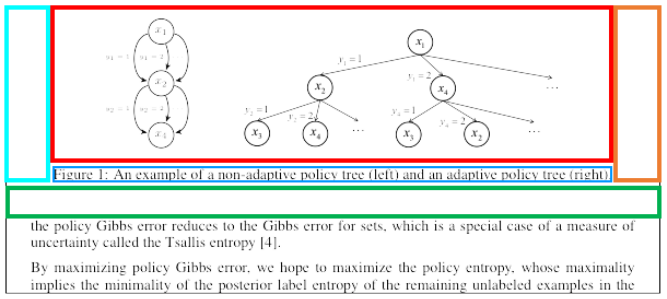
\includegraphics[width=0.48\textwidth]{pdffigures}
\caption{An example of seperation into regions}\label{fig:pdffigure}
\end{figure}


To assign captions/titles to figures or tables clustering is utilized. 
These clusters would be pruned and additional rules for increased performance.
Questions that would match up with elements in a caption can now be linked to a corresponding image which might contain useful information to answer the question.



%------------------------------------------------

\section{Text Based Knowledge Extraction}
Texts from books and other sources often contain a large amount of information. Natural languages are flexible enough to communicate complex concepts, intricate relations and more. However, AI systems currently have a hard time accessing and reasoning with the knowledge contained in texts.
\\
Even though interpreting natural language is, so far, an unsolved problem. The limited scope of solving science tests brings a solution within reach. A significant part of the knowledge can be expressed with relations like ``X causes Y'', ``X is part of Y'', ``X is an example of Y'' or ``X [verb] Y''. The algorithm by Clark et al. \cite{construction} uses a hand-crafted set of extraction rules to generate a set of expressions from the text, where relations of interest are expressed. Figure \ref{fig:extraction} shows an example of this. Extractions are a semi-formal data structure, but they can easily be translated into formal representation. Many of these rules combined form a knowledge base.

\begin{figure}
\noindent\fbox{%
    \parbox{\columnwidth}{%
       ''Mechanical energy is produced when two objects move together.''
       \center{$\Downarrow$}
       \\
(``two objects''/?x ``produce'' ``Mechanical energy'') ``when'' /CONDITION \\(``two objects'' /?x ``move'' ``'' [ ``together'' ])
    }%
}
\caption{An example of an extraction}
\label{fig:extraction}
\end{figure}

%------------------------------------------------

\section{Answering Questions}
Answering a question is a two-fold problem: The first part is actually understanding the question. A question is a query for a piece of knowledge, so the text of the question needs to be translated to a formal language. The second part is actually answering the question. Once the query is expressed in the right format, it needs to be executed on the knowledge base. Not every answer is stated explicitly in the knowledge base, so logical inference is required to combine multiple rules into a single answer. 
\subsection{Lexical analysis of questions}
The approach chosen by Krishnamurthy \cite{probseman} to parse the question is to actually reconstruct it from logical rules. The model is trained with manually translated questions. This allows the model to come up with possible rules and the likelihood that words and combinations of words translate into those rules. When the model is applied on a new question, it can look up the words and combine their corresponding rules from the bottom up. The probabilities calculated during training are used to decide at each step which of the options is the most likely.



\subsubsection{Generating rules}
Training the model comes down to constructing a probabilistic context free grammar which produces questions. This kind of grammar consists of unary rules, nonterminal rules and terminal rules. A question can be built from a grammer by repeatedly replacing unary or nonterminal symbols with other, matching, symbols untill only terminal symbols are left. A training example consists of a question ($w$)and a set of logical forms ($L$) which match the question. The goal is to learn rules which form a grammar that can produce the question. When faced with a new question, those same rules are used to build the new question. The algorithm that generates rules from a training example works as follows:
\begin{enumerate}
\item Add all rules from the training example: Add all $L$ to the grammar as a nonterminal rule (it can be seen as the starting rule), and add a unary rule $ L \rightarrow \ell $ to the grammar for every $\ell \in L$.
\item Enumerate all logical form splits: Many logical forms are a combination two independent logical rules which can be split into separate rules. For all $\ell \in L$, do a depth-first search starting at $\ell$. This involves splitting logical form $f$ into a set of $g,\, h$ pairs, adding the rules $ f \rightarrow g \enspace h$ and $ f \rightarrow h \enspace g$ to the grammar and adding $g$ and $h$ to the queue to be explored later on. Note that these rules are binary, leading to a tree structure when applied.
\item Create lexicon entries: Add a terminal rule $ f \rightarrow w$ for every combination between a word in the question and logical forms $f$ encountered during the search above
\item Allow word skipping: Add nonterminal rules which allow allow for word skipping. Add $ f \rightarrow f \enspace SKIP$ and $ f \rightarrow SKIP \enspace f$ for all logical forms and $ SKIP \rightarrow w$ for all words in the question.
\end{enumerate}

\begin{figure}[H]
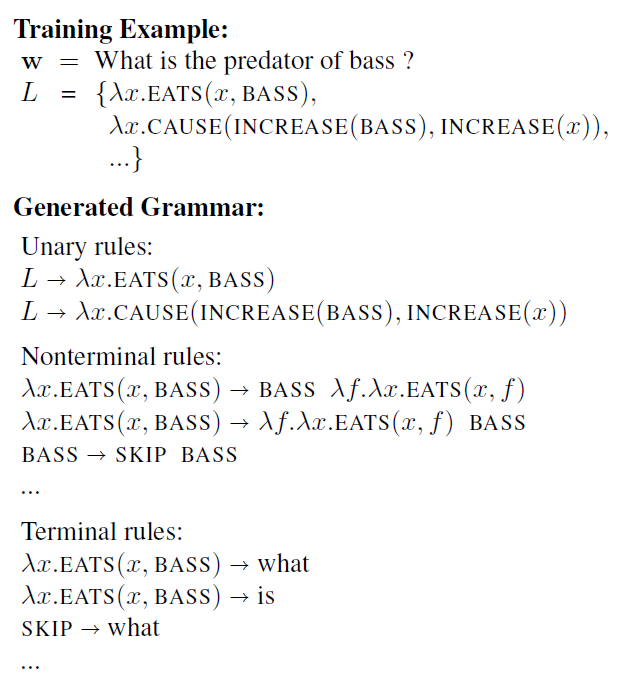
\includegraphics[width=0.48\textwidth]{rules}
\caption{The grammar generated by the algorithm from a training example}\label{fig:rules}
\end{figure}

\subsubsection{Modelling probabilities}
The generated rules from many different training examples form a grammar $G$. The production rules in $G$ can build a large amount of parse trees. To determine the most likely interpretation for a question, we need to know the probability of generating each unique parse tree. $P(t|L; \theta)$ denotes the probability of generating tree $t$ from $G$ with as root a given label $L$, and parameters $\theta$. This can in turn be broken down into a product of the probabilities of applying each rule in $t$. $ P(f \rightarrow g \enspace h; \theta)$ and $ P(f \rightarrow w; \theta)$ represent the probability of picking a replacement rule given the nonterminal $f$.

\begin{figure}[H]
\begin{center}
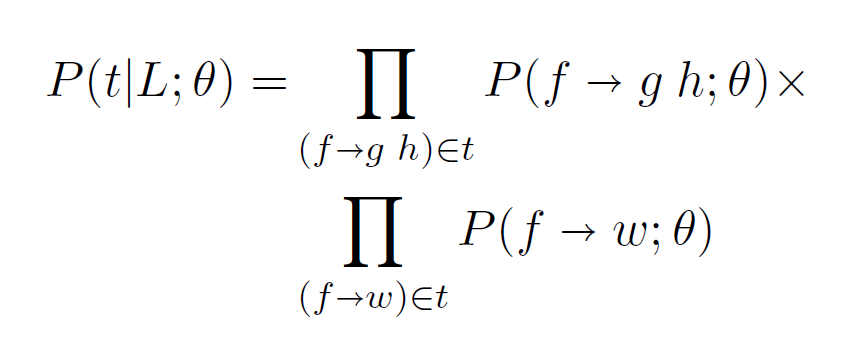
\includegraphics[width=0.4\textwidth]{prob1}
\end{center}
\label{fig:prob1}
\end{figure}

Not all of these trees build the same question, so for each specific question we're interested in all the trees with root $L$ that build a certain question $w$. This can be denoted as $P(w, t|L; \theta)$. Finally, the probability of building a question given L is:

\begin{figure}[H]
\begin{center}
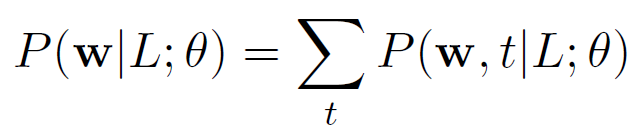
\includegraphics[width=0.3\textwidth]{coupled}
\end{center}
\label{fig:coupled}
\end{figure}

To train the model, expectation maximisation can be used. This will tweak the probabilities of applying each replacement rule in such a way that the probabilities of generating the training questions is are maximised when their labels are given. With the probabilities of applying the specific rules from grammar optimised, parser can determine the most likely parse tree by going through the building process in reverse.

\begin{figure}[H]
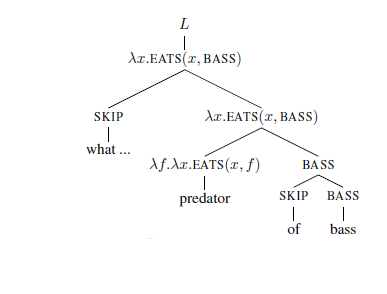
\includegraphics[width=0.48\textwidth]{parsetree}
\caption{The parse tree for the question ``What is the predator of bass?'' During training, the algorithm works from the top down to build the replacement rules. When the model is actually applied, these replacement rules are applied from the bottom up to come up with the final interpretation.}\label{fig:parsetree}
\end{figure}

\subsection{Querying the knowledge graph}
Once the meaning of the question is clear, an answer needs to be found in the knowledge base. The algorithm by Li and Clark \cite{sciencequestions} is one way to achieve that goal. After parsing the question, they extract keywords. Background knowledge is added, which results in a knowledge graph of concepts connected by the relations found in the knowledge base. These concepts are the keywords themselves, but also other related words which provide context. The questions are multiple choice, so each option is placed within that graph and connected to the other concepts. Not all of the background information that has been added is relevant in context of the given option.

 For each newly added word, a score is calculated. This score is based on the importance score ($IS$) of other keywords, and how strongly related the given word is with those keywords. Once the score has been calculated, only the most important words are kept in the graph.

\begin{figure}[H]
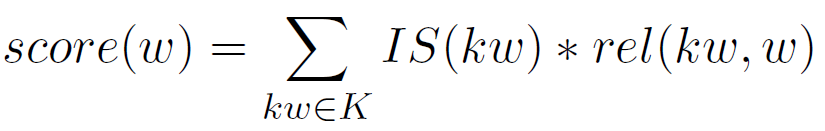
\includegraphics[width=0.48\textwidth]{score}
\end{figure}

To select the right option as the answer, a coherence value is calculated for each option. This is done by looking at all the words the option has a relationship with (i.e. they are connected on the graph), and adding strength of the relations. The option with the highest coherence value is picked as the answer.

\begin{figure}[H]
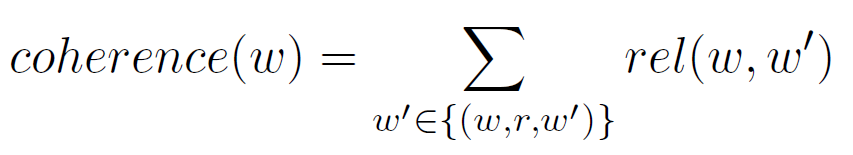
\includegraphics[width=0.48\textwidth]{coherence}
\end{figure}

\begin{figure}[H]
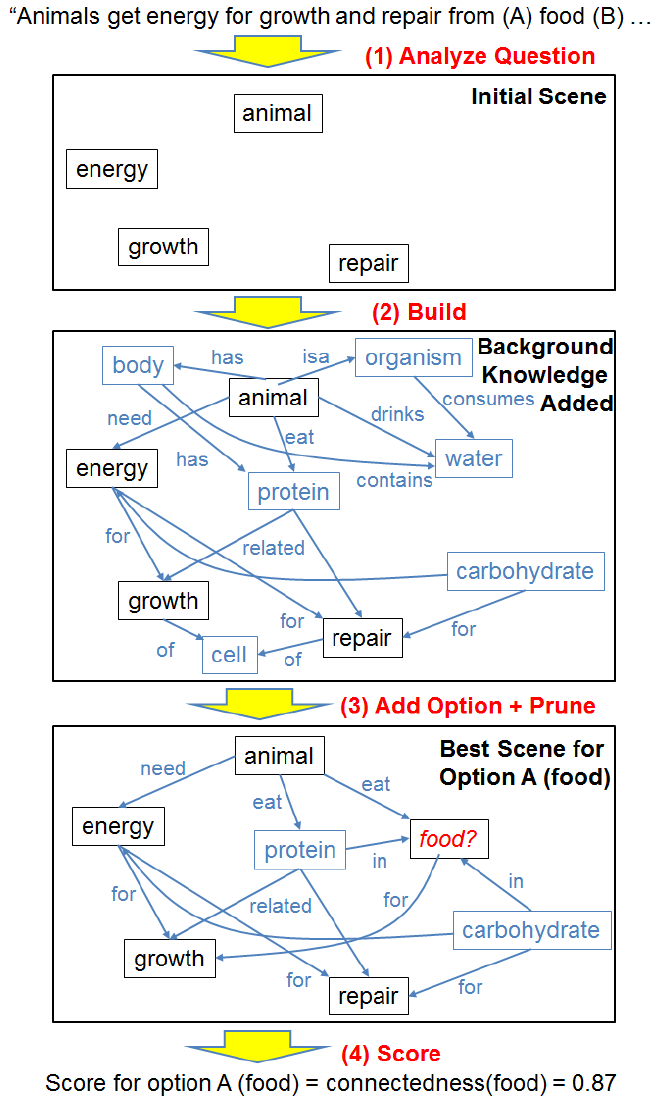
\includegraphics[width=0.48\textwidth]{graph}
\caption{An example of a question being answered using a knowledge graph.}\label{fig:parsetree}
\end{figure}








%------------------------------------------------

\section{Conclusion}

\section{Conclusion}
\label{sec:conclusion}
Our experiments show that the effectiveness of reducing the graph is highly dependent on how interconnected the graph is. The advantage of reducing the graph is not only execution time, as we expected, but it also significantly improves the quality of the initial random population for the genetic algorithm. This advantage is clear in graphs with on the order of hundreds of vertices or more, and proportional with the amount reduction that done. There are also obvious performance benefits for medium-sized graphs of several thousands of vertices. However, for larger graphs with tens of thousands of nodes, the genetic algorithm becomes ineffective when combined with the short execution times we allowed. The reduced graph still has a significant advantage, but only due to better initialization.
\par
Because of this we conclude that our graph reduction preprocessing can be very useful in certain scenarios. When graphs are highly interconnected, reducing the graph improves both the execution time and the score of the result. While the reduced search space can leave out the optimal solution, for large graphs this is not an issue. In many cases, a better solution is found in less time.

%----------------------------------------------------------------------------------------
%	REFERENCE LIST
%----------------------------------------------------------------------------------------

\bibliographystyle{plain}
\bibliography{bib}

%----------------------------------------------------------------------------------------

\end{document}
